\documentclass{article}

\usepackage{geometry}
\geometry{margin=2cm, includefoot, footskip=30pt}
\usepackage{setspace}
\usepackage{amsmath}
\usepackage{graphicx}
\usepackage{subcaption}
\usepackage{booktabs}
\usepackage{tikz}
\usepackage{siunitx}
\sisetup{
  round-mode= places,
  round-precision= 3, % decimal
}
\usepackage{multirow}
\usepackage{longtable}
\usepackage{rotating}
\usepackage[backend=bibtex, style=reading, sorting=nyt]{biblatex} %style=numeric, alphabetic, authoryear, authortitle, verbose, reading, draft
%\addbibresource{citation1}
\addbibresource{citation1.bib}
%\addbibresource{citation2.bibtex} % the file extension has to be .bib instead of .bibtex

\title{LaTeX packages}
\date{\today}

\begin{document}
\maketitle
\newpage
\doublespacing
\tableofcontents
\singlespacing
\newpage

\newgeometry{a4paper, total={6in, 8in}}
\section{Section}
Dummy text
\subsection{Subsection}
Dummy text
\section{Another Section}
Dummy text

This part can be used with package `amsmath'
\begin{equation*}
  f(x) = x^2
\end{equation*}

This part can be used with package `graphicx`
\begin{figure}[h!]
  \includegraphics[width=\linewidth]{LaTeX.png}
  \caption{LaTeX figure}
  \label{fig:LaTeX}
\end{figure}

For subfigures, package `subcaption` is needed
\begin{figure}[h!]
  \centering
  \begin{subfigure}[b]{0.4\linewidth}
    \includegraphics[width=\linewidth]{LaTeX.png}
    \caption{1}
  \end{subfigure}
  \begin{subfigure}[b]{0.4\linewidth}
    \includegraphics[width=\linewidth]{LaTeX.png}
    \caption{2}
  \end{subfigure}
  \caption{Two subfigures}
  \label{fig:LaTeX2}
\end{figure}

\newpage
\section{Tables}
\paragraph{Normal table}
\begin{tabular}{| l | c | r |}
\hline
A & B & C\\
\hline
L & C & R\\
left & center & right\\
\hline
1 & 2 & 3\\
\hline
1.01 & 2.02 & 3.03\\
\hline
1.1 & 2.002 & 3.003\\
\hline
\end{tabular}

\paragraph{booktabs}
\begin{tabular}{l  c  r}
\toprule
A & B & C\\
\midrule
L & C & R\\
left & center & right\\
1 & 2 & 3\\
\bottomrule
\end{tabular}

\paragraph{Aligned decimal}
\begin{tabular}{| S | S | S |}
\hline
1 & 2 & 3\\
\hline
1.01 & 2.02 & 3.03\\
\hline
1.1 & 2.002 & 3.003\\
\hline
\end{tabular}

\paragraph{multirow table}
\begin{tabular}{| l | c | r |}
\hline
\multirow{2}{*}{A} & B & C\\
                                & C  & R\\
\hline
L & \multirow{2}{*}{center} & \multirow{2}{*}{right}\\
left & &\\
\hline
1 & \multicolumn{2}{r |}{2}\\
\hline
\end{tabular}

\paragraph{longtable}
\begin{longtable}[l]{| l | c | r |}
\hline
A & B & C\\
\hline
L & C & R\\
left & center & right\\
\hline
\endfirsthead
\hline
A & B & C\\
\hline
L & C & R\\
left & center & right\\
\hline
\endhead
1 & 2 & 3\\
2 & 2 & 3\\
3 & 2 & 3\\
4 & 2 & 3\\
5 & 2 & 3\\
6 & 2 & 3\\
7 & 2 & 3\\
8 & 2 & 3\\
9 & 2 & 3\\
10 & 2 & 3\\
11 & 2 & 3\\
12 & 2 & 3\\
13 & 2 & 3\\
14 & 2 & 3\\
15 & 2 & 3\\
16 & 2 & 3\\
17 & 2 & 3\\
18 & 2 & 3\\
19 & 2 & 3\\
20 & 2 & 3\\
21 & 2 & 3\\
22 & 2 & 3\\
23 & 2 & 3\\
24 & 2 & 3\\
25 & 2 & 3\\
26 & 2 & 3\\
27 & 2 & 3\\
28 & 2 & 3\\
29 & 2 & 3\\
30 & 2 & 3\\
\hline
\end{longtable}

\begin{sidewaystable}[p]
\paragraph{Rotated table}
  \begin{center}
		\begin{tabular}{l  c  r}
		\toprule
		A & B & C\\
		\midrule
		L & C & R\\
		left & center & right\\
		1 & 2 & 3\\
		\bottomrule
		\end{tabular}
	\end{center}
\end{sidewaystable}
\newpage

\section{Drawing}
\begin{center}
  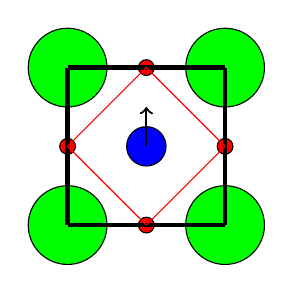
\begin{tikzpicture}
    \draw [color=black, fill=green] (-1, 1) circle(.5);
    \draw [color=black, fill=green] (1, 1) circle(.5);
    \draw [color=black, fill=green] (1, -1) circle(.5);
    \draw [color=black, fill=green] (-1, -1) circle(.5);
    \draw [color=black, fill=red] (0, 1) circle(.1);
    \draw [color=black, fill=red] (1, 0) circle(.1);
    \draw [color=black, fill=red] (0, -1) circle(.1);
    \draw [color=black, fill=red] (-1, 0) circle(.1);
    \draw [color=black, fill=blue] (0, 0) circle(.25);
    \draw [ultra thick] (-1,1) -- (1,1);
    \draw [ultra thick] (1,1) -- (1,-1);
    \draw [ultra thick] (1,-1) -- (-1,-1);
    \draw [ultra thick] (-1,-1) -- (-1,1);
    \draw [thin, color=red] (0,1) -- (1,0);
    \draw [thin, color=red] (1,0) -- (0,-1);
    \draw [thin, color=red] (0,-1) -- (-1,0);
    \draw [thin, color=red] (-1,0) -- (0,1);
    \draw [thick, -to] (0,0) -- (0,0.5);
  \end{tikzpicture}
\end{center}

These are citations \autocite[2]{PhysRevB.78.104104} and \textcite[1]{PhysRevLett.99.077601} using biblatex.
\newpage

\printbibliography

\end{document}